\documentclass[12pt, openany]{report}
\usepackage[utf8]{inputenc}
\usepackage[T1]{fontenc}
\usepackage[a4paper,left=2cm,right=2cm,top=2cm,bottom=2cm]{geometry}
\usepackage[frenchb]{babel}
\usepackage{libertine}
\usepackage[pdftex]{graphicx}
\usepackage{lastpage}
\usepackage[toc,page]{appendix}
\usepackage{hyperref}

\setlength{\parindent}{0cm}
\setlength{\parskip}{1ex plus 0.5ex minus 0.2ex}
\newcommand{\hsp}{\hspace{20pt}}
\newcommand{\HRule}{\rule{\linewidth}{0.5mm}}
\renewcommand{\appendixpagename}{}

\begin{document}

\begin{titlepage}
  \begin{sffamily}
  \begin{center}

    %Logo de l'INSA de Rouen
    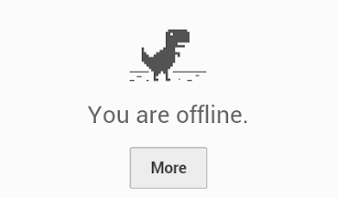
\includegraphics[scale=0.8]{./images/offlinedinosaru.png}~\\[1.5cm]

    %Titre de la matière
    \textsc{\LARGE Conception et Architecture des Systèmes d'Information}\\[2cm]

    %Type de rapport
    \textsc{\Large Monographie}\\[1.5cm]

    %Titre du sujet
    \HRule \\[0.4cm]
    { \huge \bfseries CASIFini - Le Web Offline }

    %Logo ESITPA
    \HRule \\[2cm]
    
\includegraphics[scale=0.3]{./images/disconnected.PNG}
    \\[2cm]

    \begin{minipage}{0.4\textwidth}
      \begin{flushleft} \large
      %Nom et prenom desredacteurs
        Anthony \textsc{Courtin}\\
        Alexandre \textsc{Hottin}\\
      \end{flushleft}
    \end{minipage}
    \begin{minipage}{0.4\textwidth}
      \begin{flushright} \large
      %Nom et prenom du prof
        \emph{A l'attention de :} Frederic Baucher \\
      \end{flushright}
    \end{minipage}

    \vfill

    %Date
    {\large Septembre 2015 — Janvier 2016}

  \end{center}
  \end{sffamily}
\end{titlepage}

%Table des matières
\tableofcontents{}
\newpage

\chapter{Question d'amorce}
\section{Réplication asynchrone de données}

	La réplication est un processus de partage d'informations pour assurer la cohérence de données entre plusieurs sources de données redondantes, pour améliorer la fiabilité, la tolérance aux pannes, ou la disponibilité. On parle de réplication de données si les mêmes données sont dupliquées sur plusieurs périphériques.\\

	La réplication n'est pas à confondre avec une sauvegarde : les données sauvegardées ne changent pas dans le temps, reflétant un état fixe des données, tandis que les données répliquées évoluent sans cesse à mesure que les données sources changent. 

\section{Concepts HTML5}

	\subsection{Application Cache}
		Application cache met l’application en cache et permet à l’application d’être disponible sans connexion à internet. L’utilisateur peut donc utiliser l’application en hors ligne. Il permet d’accélérer la vitesse de l’utilisation de l’application car elle est en cache et de réduire le volume de données à télécharger auprès du serveur.

	\subsection{Offline Storage} 
		Offline Storage permet de sauvegarder les données et de faire fonctionner les applications ou les jeux sans être connectés à internet.

\section{API HTML5}
	
	\subsection{Web Storage}
		Les applications web peuvent être stockées en local dans le navigateur internet de l’utilisateur. Plus performant que les cookies.

	\subsection{Web SQL Database}
		Enregistrement des données dans une base de données pouvant être interrogée en SQL.

	\subsection{Indexed Database}
		La base de données contient des valeurs et des objets hiérarchisés. Un enregistrement se compose d’une clé et d’une valeur. Un index est implémenté pour optimiser l’accès aux données.

	\subsection{File Access}
		Représentation du fichier en objet dans l’application web. L’accès aux données se fait par les objets correspondants.

\section{Bases de données}
	Les principaux types de bases de données offrant des fonctionnalités de réplication dans un contexte Web sont les suivantes :

	\begin{itemize}
		\item MySQL ;;
		\item PostgreSQL
	\end{itemize}

\chapter{Partie A}
\section{A0. Introduction}
	Le sujet du projet est: Application Web Offline.\\
	Parmi les problématiques que l'on aura à traiter on trouvera : la tolérance aux pertes partielles ou totales de connexion, la synchronisation de référentiels de données, la gestion des conflits, le stockage des données, authentification, gestion des données.

\section{A1. Mots-clés}

	\begin{itemize}
		\item HTML5 ; 
		\item Application Cache ; 
		\item Offline Storage ;
		\item Mobile ;
		\item Indexed Database \& Web SQL Database ;
		\item Réplication asynchrone de données ; 
		\item Application Web Offline ;
		\item Manifest File ;
		\item Synchronisation ;
		\item Complexité.
	\end{itemize}

\section{A2. Webographie}

	\textbf{HTML5-CSS3}, \url{http://www.html5-css3.fr/html5/tutoriel-application-web-offline-html5-cache-manifest}\\

	\textbf{Blog Nouvelles Technologies}, \url{http://www.blog-nouvelles-technologies.fr/4116/comment-faire-pour-creer-une-application-web-hors-ligne-en-html5/}\\

	\textbf{W3 Schools}, \url{http://www.w3schools.com/html/html5_app_cache.asp}\\

	\textbf{Mozilla}, \url{https://developer.mozilla.org/fr/Apps/Build/Hors-ligne}\\

	\textbf{IBM}, \url{http://www.ibm.com/developerworks/xml/library/x-html5mobile3/index.html}

\section{A3. Bibliographie}

	Rodolphe Rimelé, \textit{HTML 5 - Une référence pour le développeur web}, Eyrolles, 7 mars 2013, 727 pages.
	\begin{itemize}
		\item Chapitre 15 - Stockage des données locales (Web Storage);
		\item Chapitre 16 - Bases de données (Indexed Database \& Web SQL Database);
		\item Chapitre 17 - Applications web hors ligne.
	\end{itemize}
	~\\

	Jean-Pierre Vincent et Jonathan Verrecchia, \textit{HTML5 - De la page web à l'application web}, Dunod, 6 juillet 2011, 256 pages.
	\begin{itemize}
		\item Chapitre 10 - Application Web Offline.
	\end{itemize}
	~\\

	Peter Lubbers, \textit{Pro HTML5 Programming: Powerful APIs for Richer Internet Application Development}, APress, 1 septembre 2010, 304 pages.
	\begin{itemize}
		\item Chapitre 9 - Using the HMTL5 Web Storage API
		\item Chapitre 10 - Creating HTML5 Offline Web Application 
	\end{itemize}

\section{A4. Organisations}		

	\subsection{Tata consultancy services}
		Tata consultancy services (TCS) est une filiale du groupe Indien Tata et est classée parmis les plus importantes sociétés de services en informatique au monde. 
		Son modèle de livraison de réseau mondial, Global Network Delivery Model, permet de répondre aux besoins de ses clients le plus rapidement possible.
		L’activité de TCS va du conseil jusqu’à la mise en oeuvre et au suivi des systèmes. De plus, il est possible pour les clients d’externaliser le processus métier ou la mise en place de services d’ingénierie.
		En ce qui concerne la participation de TCS dans le domaine du Web Offline, elle a publié un Livre blanc disponible à cette adresse : 
		\url{http://www.tcs.com/SiteCollectionDocuments/White%20Papers/TEG_Whitepaper_Developing_Offline_Web_Application_Using_HTML5_0212-1.pdf}

	\subsection{W3C}
		Le World Wide Web Consortium est une organisation à but non lucratif s’occupant de la standardisation dans le domaine de l’informatique. Elle fut fondée en 1994 dans le but de promouvoir les technologies du Web.
		La gestion du W3C est assurée par le MIT, l’ERCIM, l’université Keio et l’université Beihang. 
		Le W3C est à l’origine de nombreux standads dans le domaine du Web. On peut notamment citer XHTML, SVG, SPARQL et HTML.
		En ce qui concerne la participation du W3C dans le domaine du Web offline, cette dernière a publier une note de groupe de travail disponible à l’adresse suivante :
		\url{http://www.w3.org/TR/offline-webapps/}

	\subsection{Mozilla Foundation}
		La Mozilla Foundation est une organisation à but non lucratif créé le 15 juillet 2003 et situé à Mountain View en Californie. Son but est de développer et de publier des logiciels libre de droit. 
		La fondation a créé un site web appelé Mozilla Developer Network  (MDN) qui regroupe de la documentation sur les technologies Web telles que HTML, CSS et Javascript.
		En ce qui concerne la participation de la Mozilla Foundation dans le domaine du Web offline, cette dernière a publier une documentation disponible à l’adresse suivante :
		\url{https://developer.mozilla.org/fr/Apps/Build/Hors-ligne}

\section{A5. Facteurs}
	
	\begin{itemize}
		\item Functionality $->$ Interoperability (1)
		\item Portability $->$ Adaptability (2)
		\item Reliability $->$ Recoverability (3)
	\end{itemize}

\section{A6. Indicateurs}
	
	\begin{itemize}
		\item Operation Time
		\item Number of Functions
		\item Data exchangeability (data format-based) (1)
		\item System software environmental adaptability (adaptability to OS, network software and cooperated application software) (2)
		\item Restoration effictiveness (3)
	\end{itemize}

\section{A7. Références théoriques}

	\subsection{Load Everything pattern}
		\begin{itemize}
			\item L’application charge toutes les données dont l’utilisateur a besoin d’utiliser directement
			\item L’utilisateur utilise les données stockées localement
			\item Le processus de chargement peut être très long suivant la connexion de l’utilisateur et la quantité de données à télécharger
		\end{itemize}

	\subsection{Caching pattern}
		\begin{itemize}
			\item L’application requête les données au serveur lorsque l’utilisateur en fait la demande et les stocke au cas où l’utilisateur en aurait encore besoin
			\item On peut citer les applications de messagerie qui stockent un certain nombre de mail, les applications de streaming musical ou bien celles utilisant une 			\item carte
			\item Il faut que l’application garde le cache à jour afin que l’utilisateur ne soit pas en retard par rapport à ce qu’il y a sur le serveur
		\end{itemize}

	\subsection{Selectiveness pattern}
		\begin{itemize}
			\item Ce pattern fonctionne comme le second à l’exception que l’utilisateur a le choix de ce qu’il souhaite mettre en cache
		\end{itemize}

\chapter{Partie B}
\section{B1. Approches techniques}

	L'intérêt du web offline est de permettre à un utilisateur d’utiliser ses applications habituellement connectées à internet (boite mail, streaming musical …) ou de consulter ses pages web préférées (casisbelli …), le tout, en étant hors-ligne. Cette technologie s’est principalement développée grâce à l’augmentation du nombre de smartphones et de tablettes. \\

	Afin de pouvoir utiliser un site web ou une application hors ligne, nous devons connaître l’état de connexion de l’utilisateur, c’est-à-dire, savoir s’il est connecté à internet ou non \textit{(pattern Message Endpoint)}. Cette étape est généralement réalisée à l’aide de fonctions de type javascripts en utilisant notamment : navigator.onLine. Une fois que nous avons pris connaissance de l’état de connexion de l’utilisateur, nous devons spécifier quelles sont et où sont situés les informations nécessaires afin d’afficher correctement le site internet ou le contenu de l’application. Cette étape passe généralement par la création d’un fichier appelé Cache Manifest et enregistré généralement sous le nom offline.manifest. Voici un exemple de fichier :\\

	CACHE MANIFEST\\
	angular.min.js\\
	bootstrap.min.js\\
	styles-perso.css\\
	jquery-1.4.min.js\\
	offline.js\\
	index.html\\
	exercices.html\\
	contact.html\\

	Il faut ensuite lier ce Cache Manifest à nos pages html de la manière suivante : \textit{$<html manifest="offline.manifest">$}\\

	Il est important de noter que les exemples donnés ci-dessus et par la suite de cette partie reposent sur l’utilisation de la technologie Application Cache. Il existe une autre technologie nommée Service Worker que nous développerons dans la partie suivante.\\

	Ensuite, il est important de stocker les données localement afin d’avoir accès aux données et de pouvoir utiliser correctement le site web ou l’application \textit{(pattern Message Store)}. \\

	Pendant l’utilisation, il est nécessaire de veiller à enregistrer les données régulièrement dans la base de données locale au risque de perdre des données dans le cas contraire. La solution la plus simple à mettre en place est la sauvegarde du DOM des pages web à l’aides des objets suivants :

	\begin{itemize}
		\item window.sessionStorage pour sauvegarder pendant la période de Session
		\item window.localStorage pour sauvegarder pour une période plus importante
	\end{itemize}
	~\\

	Dans tous les cas, ces objets offrent le même type de fonction permettant d'accéder aux données, de sauvegarder ces dernières ou de les supprimer facilement.\\

	Une fois que la connexion à internet est rétablie, les données stockées en locale doivent être synchronisées avec le serveur distant \textit{(pattern Messaging)} \textit{(pattern Message Endpoint)} \textit{(pattern Message Filter)}. Il faut donc prévoir de créer une queue des données pour être cohérent avec l’évolution des données en mode hors ligne \textit{(pattern Resequencer)}. La transaction des données doit être vérifiée et réussie pour pouvoir passer à la transaction suivante \textit{(pattern Guaranteed Delivery)}. Si la connexion à internet coupe pendant une transaction, c’est comme ci elle n’avait pas été réalisée et doit donc être refaite lors d’une nouvelle connexion à internet. De plus, si des modifications ont été réalisées sur le serveur distant entre deux connexions, ces dernières vont être téléchargées vers le dossier de stockage local \textit{(pattern Shared Database)}.\\

La figure~\ref{schema} explique l'architecture d'une application en web offline.

 \begin{figure}[H]
  \centering
  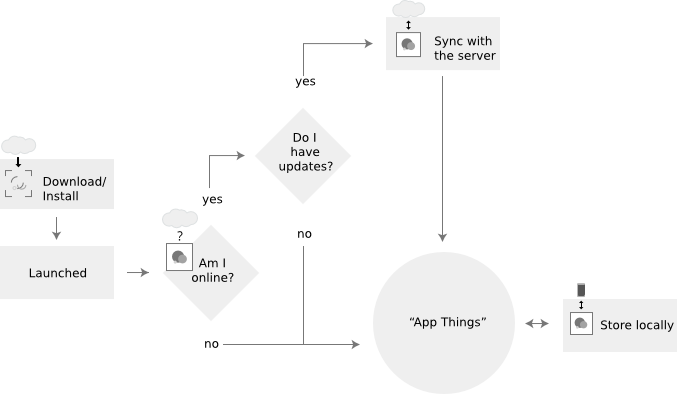
\includegraphics[width=18cm]{./images/schema.png}
  \caption{Schéma explicatif}
  \label{schema}
 \end{figure}

\section{B2. Solutions technologiques}

\section{B3. Description technique}

Détecter l'état de connexion à internet :
	\begin{itemize}
		\item offline.js
		\item failsafe.js
	\end{itemize}
	~\\

Stockage des informations nécessaire à l’affichage :
	\begin{itemize}
		\item manifest
	\end{itemize}
	~\\
	
Stockage des données :
	\begin{itemize}
		\item localForage
		\item localStorage
	\end{itemize}
	~\\

\section{B4. Benchmark}

	\begin{itemize}
		\item Functionality $->$ Interoperability
			\begin{itemize}
				\item Data exchangeability (data format-based)
			\end{itemize}
		\item Portability $->$ Adaptability
			\begin{itemize}
				\item System software environmental adaptability (adaptability to OS, network software and cooperated application software)
			\end{itemize}
		\item Reliability $->$ Recoverability
			\begin{itemize}
				\item Restoration effictiveness
			\end{itemize}
		\item Operation Time
		\item Number of Functions
	\end{itemize}
	~\\

\section{B5. Work Breakdown Structure}

 \begin{figure}[H]
  \centering
  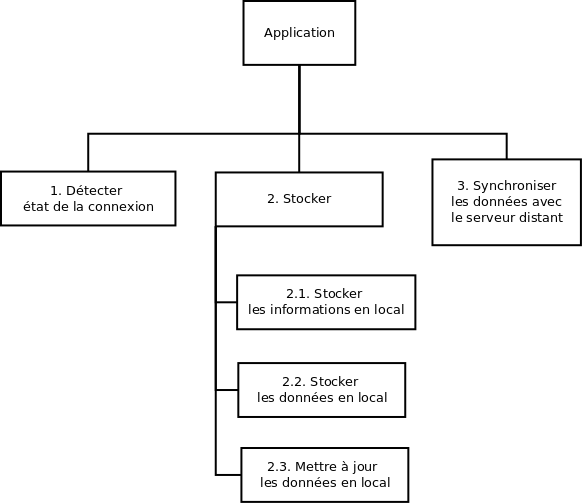
\includegraphics[width=18cm]{./images/wbs.png}
  \caption{Work Breakdown Structure}
 \end{figure}


% \chapter{Etat de l'art}
% \input{etat_de_l_art.tex}

% \chapter{Conclusion}
% \input{conclusion.tex}

% \chapter{Bibliographie}
% \input{references.tex}

% \chapter{Annexes}
% \input{annexe.tex}

%Tables des tableaux
% \listoftables 
%Table des figures
\listoffigures

\end{document}
